With the high level design and primary component selection complete, detailed design of the VNA could begin. KiCad was used for all steps of the PCB design process, as it is a powerful free and open source EDA tool which is extensively used in the open source hardware community. For firmware, System Workbench for STM32 was utilised, as it provides open source tools such as GCC for Cortex-M cross compiling, OpenOCD for programming and debugging, precompiled and integrated in an Eclipse IDE, which makes getting firmware development started with a completely open source flow easy.

\subsection{Schematic Capture}
The first step in PCB design is schematic capture, where abstract representations of the components are joined together in a way which makes it easy to read and determine the desired functionality of the device. Due to development boards being designed earlier in the process, certain components such at the MAX2871 PLL, filter bank, and gain control circuitry were easily ported over into the new schematic, however due to issues such as a new amplifier needing to be designed in, along with the programmable attenuator being out of stock, changes were required to ensure that all components were able to be sourced in time, along with preforming as desired.

Other components such as the STM32 microcontroller, dual directional couplers, numerous status LEDs, and an auxiliary USB connection for powering DUTs and ECal units were also added to ensure that all required hardware was on device. Additionally numerous design for test additions such as 0 ohm resistors and DNP components, test points on all key signals, additional components in the PLL loop filter to allow an alternative PLL to be utilised, user addressable LEDs, unused pints being broken out, power rail LEDs, numerous ground points along with a unused UART connection were all designed in to make bring-up of the board as easy as possible. The completed schematic can be found in Appendix \ref{appen:vna_design_files}, Figures \ref{fig:vna_schematic_overview} through \ref{fig:vna_schematic_power}.

\subsection{Layout Planning}
Before the PCB layout can begin, there are a few key steps and decisions which need to made which will place constraints on the design of the PCB. Firstly, component footprints were associated with the relevant schematic symbols, with footprints being designed where KiCad did not have them in the standard library. Furthermore 3D models for every component were either loaded from KiCad, sourced from the distributor, or drawn from mechanical drawings, as this would allow for mechanical fit with an enclosure to be confirmed later in the design process. 

With all the components imported into CAD, the approximate size of the PCB was able to be determined. This allowed for COTS aluminium case options to be explored, and once an enclosure was found which was large enough for the PCB to fit, the exact dimensions of the PCB were able to be fixed to that dimension, allowing the positioning of connectors, mounting holes, and other key features of the PCB to be placed. 

The PCB stackup and manufacturer also needed to be determined, as this plays a key role in the cost of the boards, along with key PCB features such as minimum space / trace, via size, and the with of a 50 ohm microstrip trace. Due to cost and prior experience, JLCPCB was chosen as the manufacturer, and their 4 layer FR4 "JLC7628" stackup (Table \ref{table:pcb_stackup}) was chosen as it is a very common stackup well suited to the feature and component sizes used by the components, along with the ability for it to be ordered from other manufacturers with ease. Furthermore, a Signal / GND / PWR / Signal configuration would be designed for during layout, with flood fills of ground on layers 1 and 4. 

\begin{table}[H]
	\centering
	\caption{Chosen PCB stackup}
	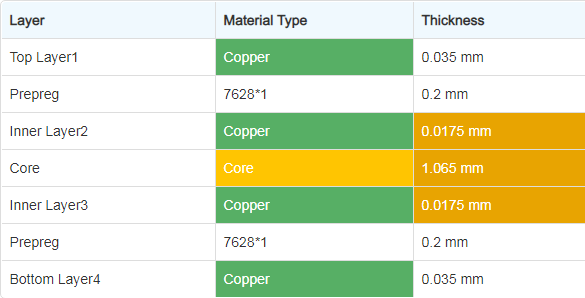
\includegraphics[width=0.8\linewidth]{jlc_stackup.png}
	\label{table:pcb_stackup}
\end{table}

Other key feature sizes for the chosen stackup and manufacturing process are outlined in Table \ref{table:pcb_specs}. It should be noted that whilst JLCPCB are able to do quite small trace / space and via drill size, 6 / 6 trace / space and 0.25 / 0.5 drill / via were chosen for the design, as this would allow it to be fabricated at common fabricators such as OSHPark and PCBWay without paying for advanced processes. 
\begin{table}[H]
	\caption{Key specifications of PCB design rules and feature size}
	\label{table:pcb_specs}
	\centering
	\begin{tabular}{|c|c|}
		\hline
		\textbf{Feature}                          & \textbf{Dimension} \\ \hline
		Min Trace / Space                         & 0.15 mm (6 mil)   \\ \hline
		Min Via Drill Size                        & 0.25 mm (10 mil)     \\ \hline
		Min Via Diameter                          & 0.5 mm (20 mil)   \\ \hline
		50 $\Omega$ Microstrip Width              & 0.29 mm (11.5 mil) \\ \hline
		Blind / Buried / Micro Via                & Not Available \\ \hline
	\end{tabular}
\end{table} 

\newpage
\subsection{PCB Layout}
Given the mechanical dimensions, stackup, and design rules have be determined, these parameters can be loaded into KiCad and the PCB can be laid out. An image of the laid out board can be found in Figure \ref{fig:pcb_layout}, with a 3D render available in Figure \ref{fig:pcb_render}.

Given the operating frequencies seen on the board, a number of key layout considerations were taken into account to ensure optimal function of the board, and are detailed below.
\begin{itemize}
	\item \textbf{50 $\Omega$ RF Traces} need to be kept along the signal path to ensure a good match between components, and this is achieved on this board through using a 0.29 mm microstrip on layer 1 over a continuous ground pour on layer 2. 
	\begin{itemize}
		\item Furthermore, compensation for extra capacitance introduced under the large pads of the directional couplers and SMA connectors need to occur, as otherwise there will be added capacitance which will decrease the match of the transmission line. This can be seen in Figure \ref{fig:pcb_cap_comp}, where the ground fill has been removed to significantly reduce the inter-planar capacitance between layers 1 and 2, to ensure a consistent characteristic impedance. 
		\item When a layer change is required for the RF signal, care must be taken to ensure there is a low impedance path between reference layers. This can be seen on the first directional coupler as shown in Figure \ref{fig:pcb_layer_change}, where the RF travels from the bottom left on layer 1, through a via to layer 4, and back to layer 1 in the top right hand corner. Stitching vias can be seen close to the signal via to ensure a low inductance path between the two reference planes, along with the signal vias being optimised to have a 50 $\Omega$ impedance to reduce impedance discontinuity. 
		
		Unfortunately a mistake was made during layout in that the signal was routed on layer 4 instead of 3, as with the signal on 4 it's reference plane is layer 3, VCC, which does not have a low inductance path to layer 2, as the closets decoupling caps are located in the top left of the image, near the 8 pin DFN IC. Ideally the signal would have been routed on layer 3,  allowing the ground pour on layer 4 to be the reference plane, with the multiple vias providing a low inductance path between the two planes. Fortunately, due to upper bounds of the frequencies seen on the board at 1.25 GHz, this is not a major issue which has caused issues with the function of the device. 
		\item Low impedance between layers was also ensured through the use of ample stitching vias, both around the signal path and the entire board. 
	\end{itemize}
	\item \textbf{EMI Reduction} is crucial to ensure that there is no coupling of unwanted signals onto the key signals. This has been achieved by routing the digital signals on the left side of the board, allowing the RF and analog signals from the AD8302 to have as much clearance as possible from the digital signals. Furthermore, the output drivers on the STM32 were set to a low slew rate, as this will decrease the frequency content seen when a signal is switched. 
	\item \textbf{Power Integrity} was achieved through the use of linear regulators to decrease noise on the power rails, low inductance connections to components through large power planes and multiple vias when changing layers to ensure the added inductance is kept to a minimum. Furthermore, ensuring the decoupling capacitors specified in application notes for each component are placed close the power pins, with the smaller capacitors closer to the pin, and a dedicated via for each capacitor placed as close as possible to the pad ensures that the impedance and noise seen at the power pin to each component is kept at a minimum, which leads to optimum performance of the IC and minimal coupling of noise onto the RF and analog signals.
	\item \textbf{Following reference layouts} ensured that the device would preform as specified on the data sheet, along with being able to rule out bad component placement and routing as possible causes for improper function of device. Where reference designs were not available, best RF layout practices including those described above were utilised to ensure optimal performance of the device.  
\end{itemize} 

\begin{figure}[H]
	\centering
	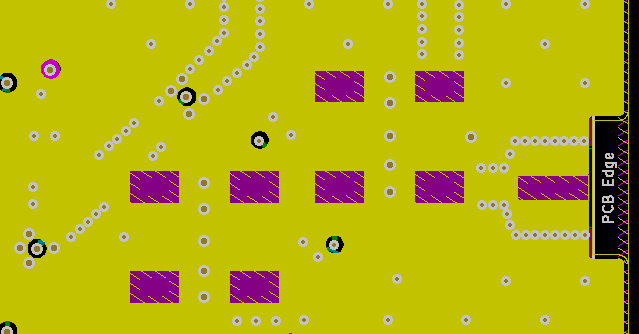
\includegraphics[width=0.6\linewidth]{ground_cutouts.png}
	\caption{Ground cut-outs under large pads to reduce inter-planar capacitance and ensure a 50 $\Omega$ transmission line}
	\label{fig:pcb_cap_comp}
\end{figure}

\begin{figure}[H]
	\centering
	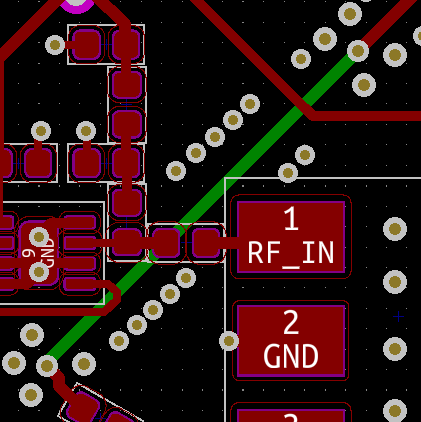
\includegraphics[width=0.4\linewidth]{layer_change.png}
	\caption{Layer change for on the signal path}
	\label{fig:pcb_layer_change}
\end{figure}

\begin{landscape}
	\begin{figure}[H]
		\centering
		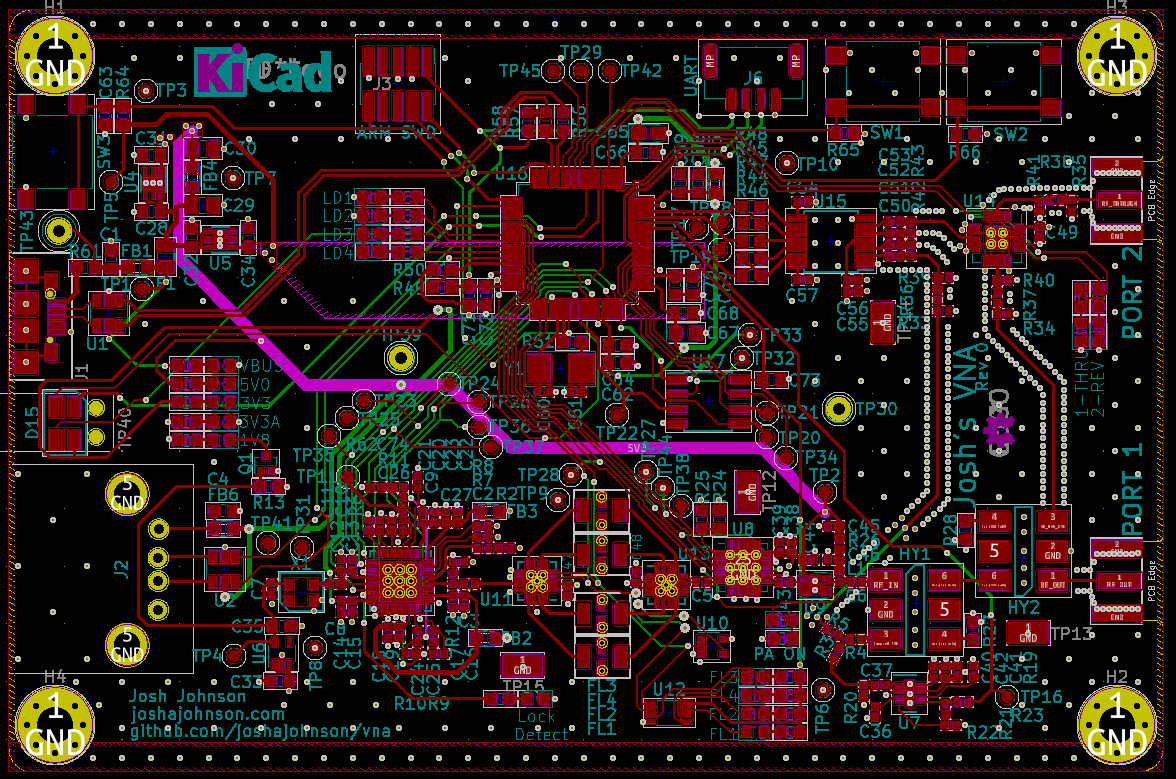
\includegraphics[width=\linewidth]{pcb_layout.png}
		\caption{PCB Layout, with Red = Layer 1, Yellow = Layer 2, Pink = Layer 3, Green = Layer 4. Flood fill of each layer is not shown.}
		\label{fig:pcb_layout}
	\end{figure}

	\begin{figure}[H]
		\centering
		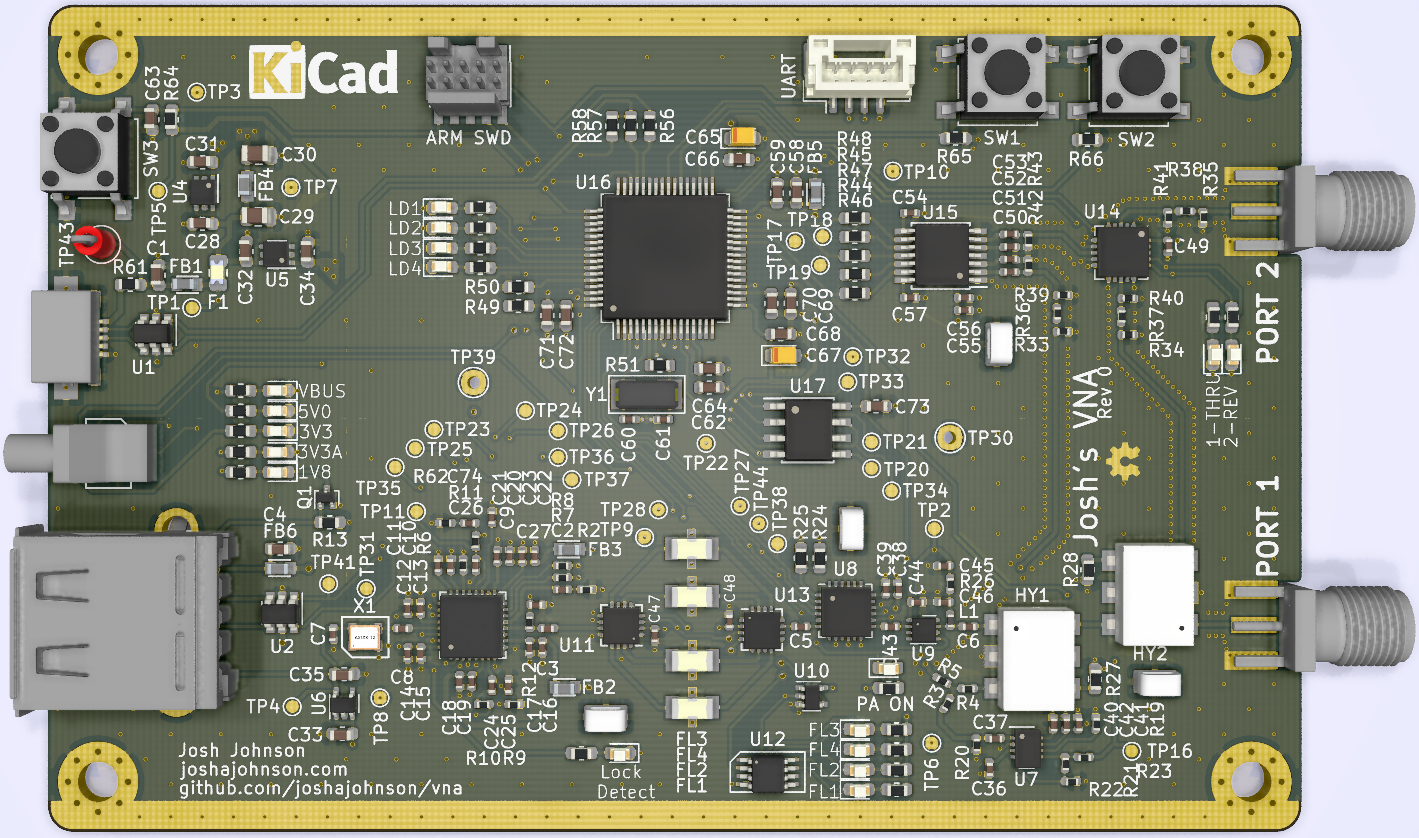
\includegraphics[width=\linewidth]{thirdDayRender.png}
		\caption{3D render of the PCB}
		\label{fig:pcb_render}
	\end{figure}
\end{landscape}

\subsection{Mechanical Design}
To ensure there will be no mechanical clearance issues, a STEP was exported from KiCad in to Fusion360 and placed into a model of the extrusion, and is was seen that there were no mechanical issues. Having the 3D model in MCAD, together with the decision to use an extruded aluminium enclosure results in easy design of custom front and rear panels, as key features from the 3D model can be referenced when designing cut-outs for the connectors and light pipe. DXFs were exported from Fusion360 back into KiCad where they had silkscreen added, and they were then sent off to be manufactured with the main VNA PCB. Renders of the front and rear panels can be found in Figures \ref{fig:pcb_front_render} and \ref{fig:pcb_rear_render}, and the assembled VNA without the top extruded section in Figure \ref{fig:pcb_assembled}.

\begin{figure}[H]
	\centering
	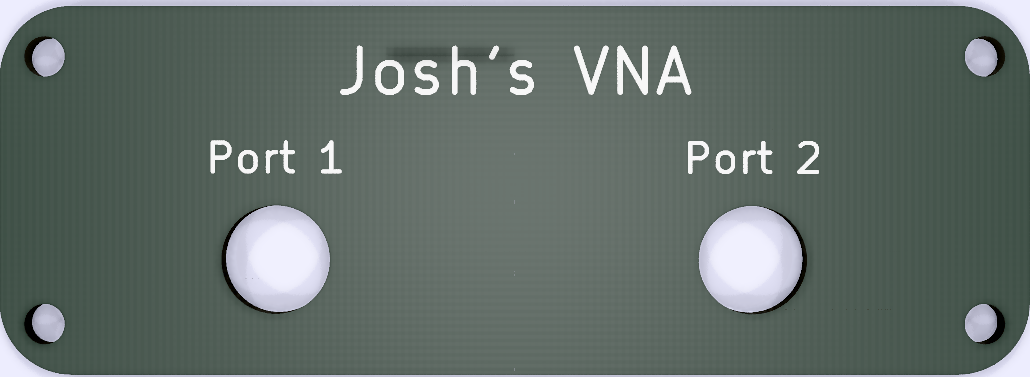
\includegraphics[width=0.8\linewidth]{frontPanel.png}
	\caption{Render of the VNA Front Panel}
	\label{fig:pcb_front_render}
\end{figure}

\begin{figure}[H]
	\centering
	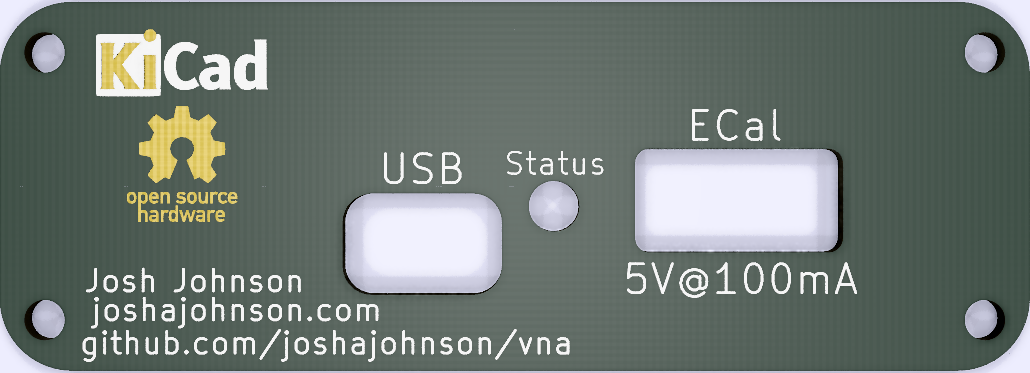
\includegraphics[width=0.8\linewidth]{rearPanel.png}
	\caption{Render of the VNA Rear Panel}
	\label{fig:pcb_rear_render}
\end{figure}

\begin{figure}[H]
	\centering
	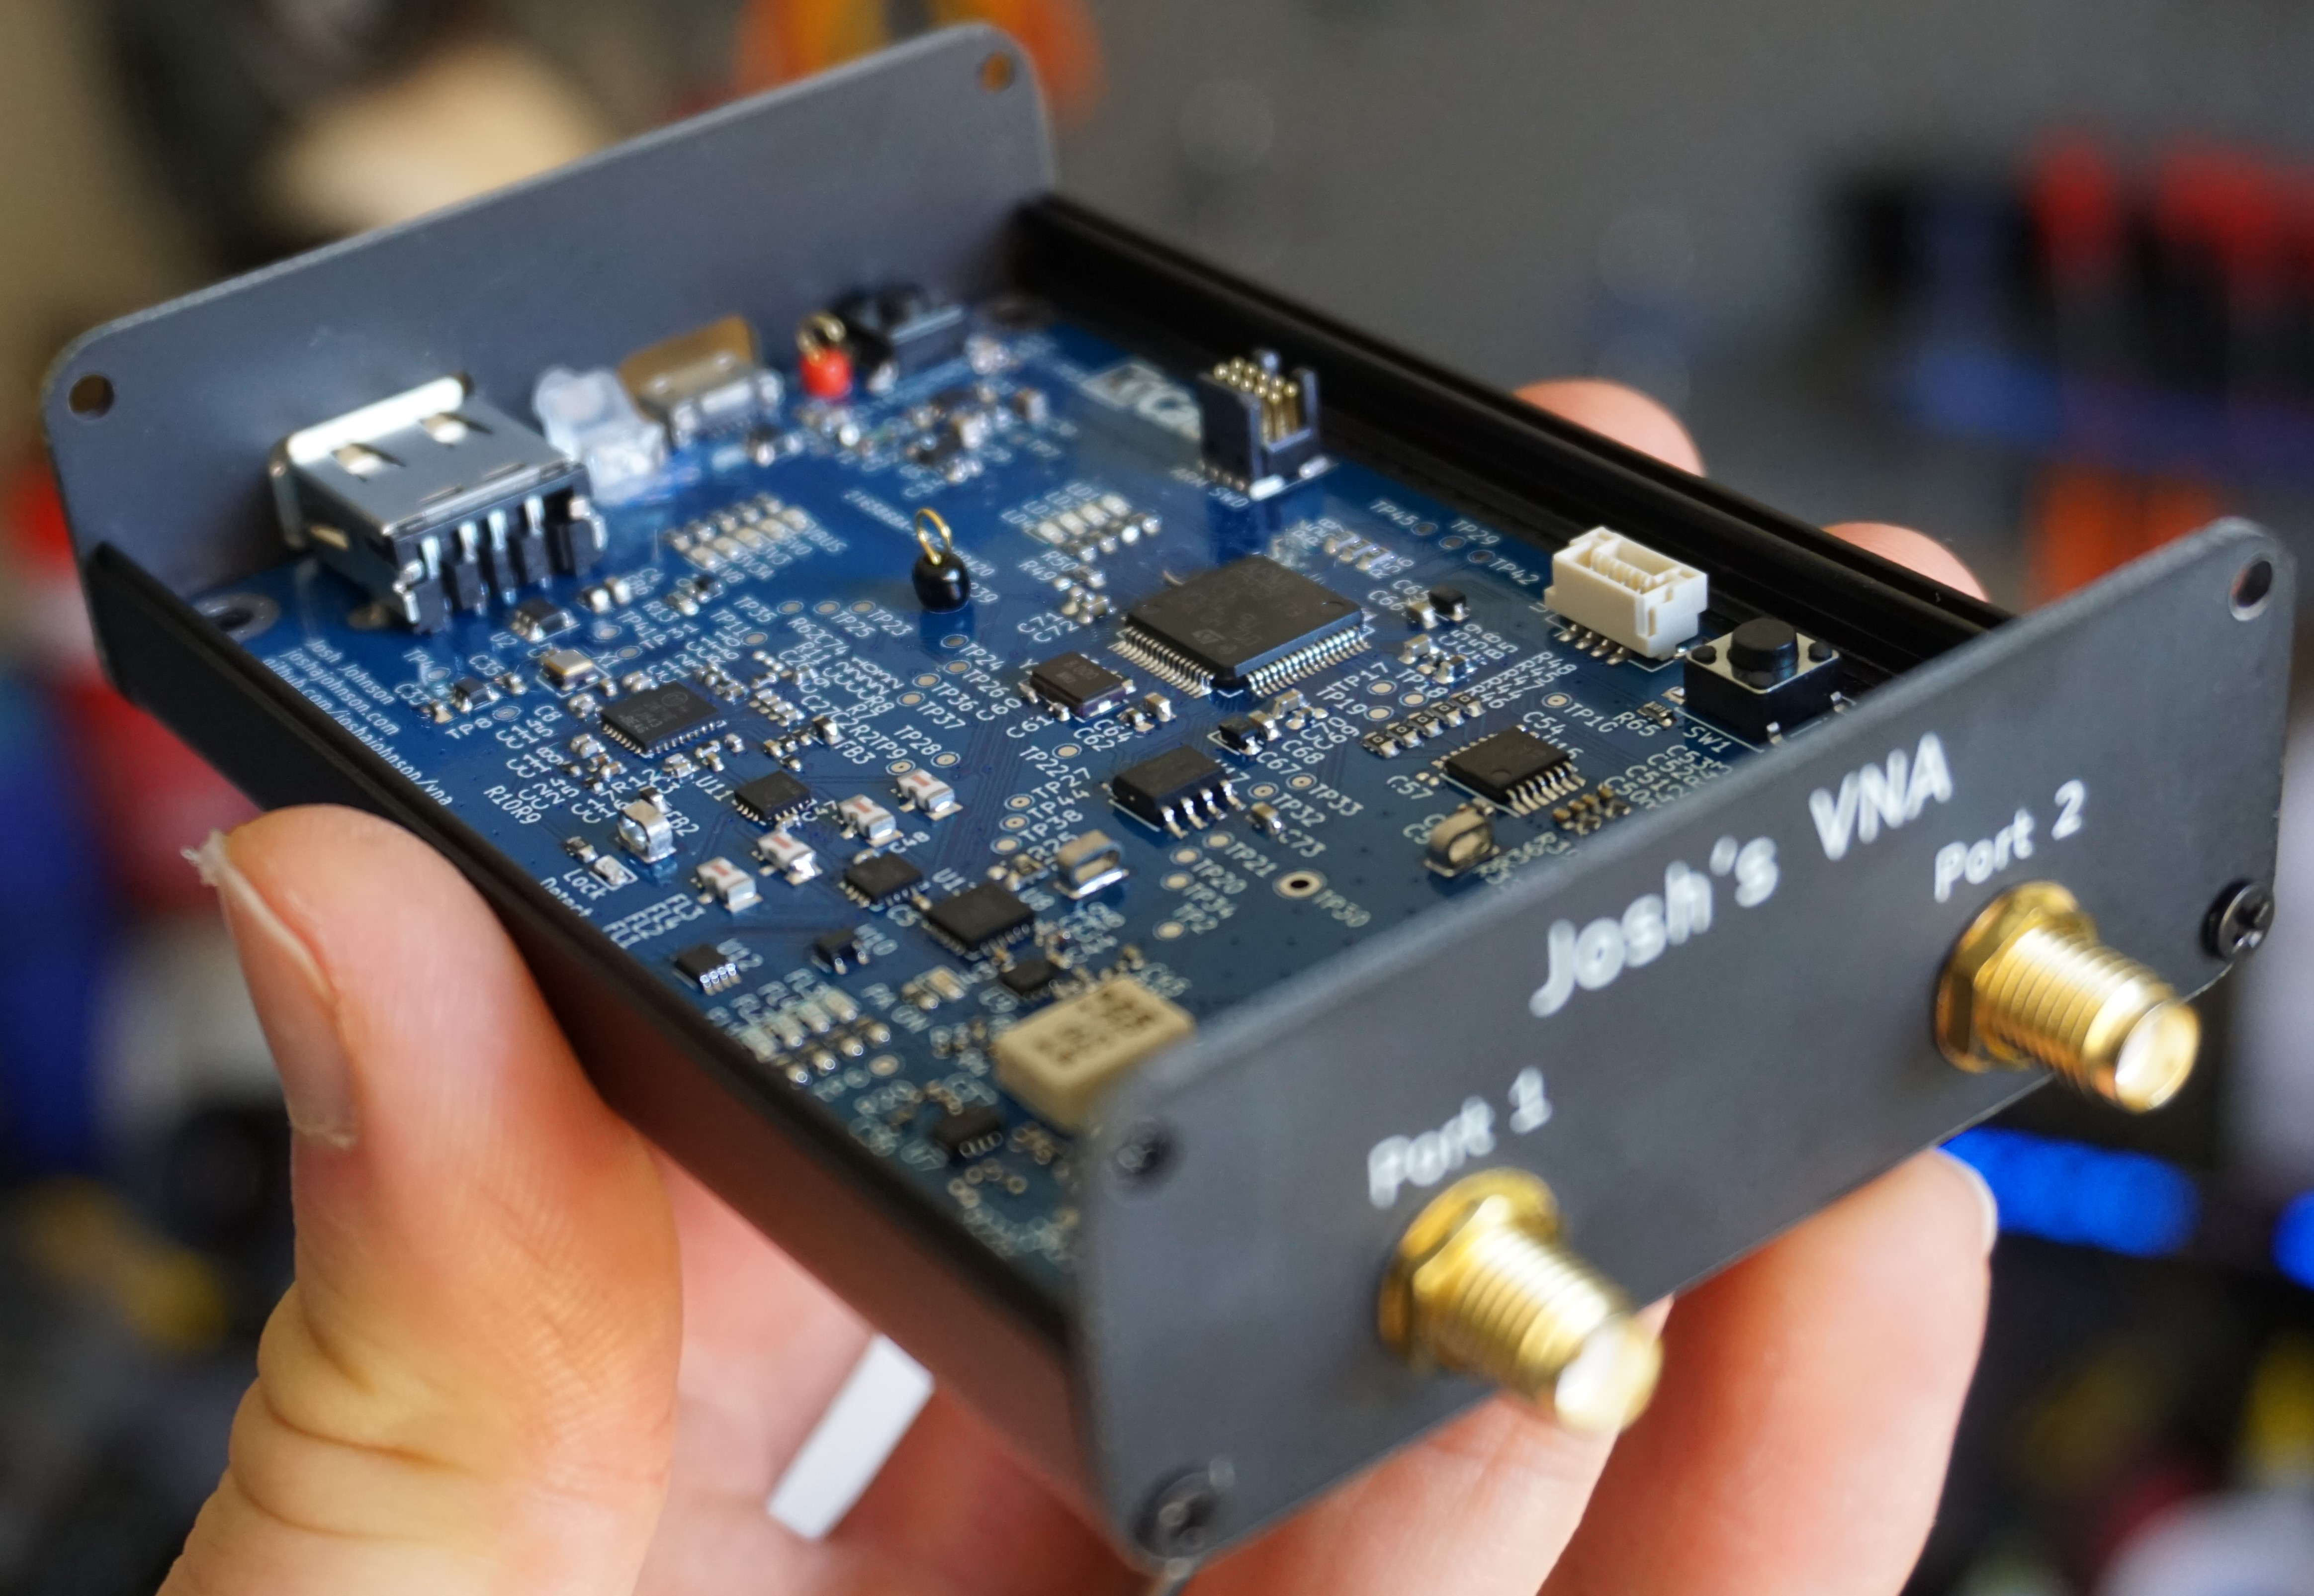
\includegraphics[width=\linewidth]{assembledVNA.jpg}
	\caption{Assembled VNA in enclosure, with top section removed}
	\label{fig:pcb_assembled}
\end{figure}

\subsection{Assembly + Bill of Materials}
Upon arrival of assembled PCBs and solder paste stencil, assembly was undertaken. This followed a fairly standard SMT process, with solder paste being deposited onto the PCB through the use of a stencil, placement of components under a microscope due to their size (down to 0402 and 0.5 mm QFN), and reflow in a reflow oven. Rework was required for a few components due to tomb stoning, along with some shorted pins on the QFNs, and hand soldering of the through hole components and SMA connectors. The board was then cleaned in an ultrasonic cleaner to remove any remaining flux, and left to dry for an hour in the reflow oven. This process went quite smoothly with the whole process taking less than 6 hours from start to finish. 

Table \ref{table:BOM} outlines the cost to manufacture one VNA, with removal of components such as debug headers and ground test points which are only required on the development boards. It should be noted that the per board cost at quantity 10 is reduced to \$204.78 due to the cost of PCBs being split between multiple boards and a slight reduction in component price, and that if free samples are requested from Analog Devices and Maxim and no case is utilised, the cost of assembling a VNA can be as little as \$185.37. Pricing is correct as of 10/10/19.


\begin{table}[H]
	\caption{Bill of Materials for VNA}
	\label{table:BOM}
	\centering
	\begin{tabular}{|c|c|c|c|c|}
		\hline
		\textbf{Quantity} & \textbf{Part Number}       & \textbf{Description}     & \textbf{\begin{tabular}[c]{@{}c@{}}Price Each \\ (\$AUD)\end{tabular}} & \textbf{\begin{tabular}[c]{@{}c@{}}Cost per Board \\ (\$AUD)\end{tabular}} \\ \hline
		1                 & MAX2871                    & PLL with VCO             & 18.95                                                                 & 18.95                                                                     \\ \hline
		1                 & ASTXR-12         & Reference Clock          & 4.75                                                                  & 4.75                                                                      \\ \hline
		2                 & PE42440                    & SP4T Switch              & 1.93                                                                  & 3.87                                                                      \\ \hline
		1                 & LFCN-105+                  & Low Pass Filter          & 15.27                                                                 & 15.27                                                                     \\ \hline
		1                 & LFCN-225+                  & Low Pass Filter          & 11.45                                                                 & 11.45                                                                     \\ \hline
		1                 & LFCN-400+                  & Low Pass Filter          & 11.45                                                                 & 11.45                                                                     \\ \hline
		1                 & LFCN-1000+                 & Low Pass Filter          & 7.61                                                                  & 7.61                                                                      \\ \hline
		1                 & TRF37A75                   & Power Amplifier          & 2.84                                                                  & 2.83                                                                      \\ \hline
		1                 & SKY12347-362LF             & Attenuator  & 10.04                                                                 & 10.04                                                                     \\ \hline
		2                 & ADC-15-4+                  & Directional Coupler      & 19.21                                                                 & 38.43                                                                     \\ \hline
		1                 & AD8319                     & Log Power Detector       & 8.69                                                                   & 8.69                                                                       \\ \hline
		1                 & AD8302                     & Gain Phase Detector      & 45.10                                                                   & 45.10                                                                       \\ \hline
		1                 & F2923                      & SPDT RF Switch           & 8.20                                                                  & 8.20                                                                      \\ \hline
		2                 & SMA                        & DUT Connector            & 2.12                                                                  & 4.24                                                                      \\ \hline
		1                 & Micro USB                  & Connection to PC         & 0.12                                                                  & 0.12                                                                      \\ \hline
		1                 & USB A                      & External Connection & 0.42                                                                  & 0.42                                                                     \\ \hline
		2                 & LP5912                     & 3V3 LDO                  & 2.01                                                                 & 4.02                                                                     \\ \hline
		1                 & MIC5366-1.8                & 1V8 LDO                  & 0.37                                                                  & 0.37                                                                      \\ \hline
		1                 & Polyfuse                   & Input protection   & 0.39                                                                  & 0.39                                                                      \\ \hline
		2                 & TPD2S017                   & ESD Protection           & 1.05                                                                  & 2.11                                                                      \\ \hline
		1                 & STM32F373              & Microcontroller           & 8.87                                                                 & 8.87                                                                      \\ \hline
		1                 & 8 MHz Crystal              & For MCU                  & 0.83                                                                  & 0.83                                                                      \\ \hline
		1                 & RGB LED                    & Status LED               & 0.88                                                                  & 0.88                                                                      \\ \hline
		1                 & Assorted Capacitors        &                          & 2.20                                                                    & 2.20                                                                        \\ \hline
		1                 & Assorted Passives &                          & 1.10                                                                    & 1.10                                                                        \\ \hline
		1                 & VNA PCB                    & (Price for 5)            & 45.67                                                                 & 45.67                                                                     \\ \hline
		1                 & Enclosure                  &                          & 8.28                                                                  & 8.22                                                                      \\ \hline
		2                 & Front/Rear Panels         & (Price for 5)            & 3.26                                                                  & 6.53                                                                      \\ \hline
		1                 & Light Pipe                 &                          & 0.98                                                                   & 0.98                                                                       \\ \hline
		&                            &                          &                                                                        &                                                                            \\ \hline
		&                            &                          & Total Cost                                                             & 272.88                                                                    \\ \hline
	\end{tabular}
\end{table} 

\subsection{Board Errata}

\subsection{ECal Design}


\subsection{Firmware Development}

\subsection{Software Development}